
\begin{figure}
\centering
\begin{subfigure}[b]{.4\textwidth}
\centering
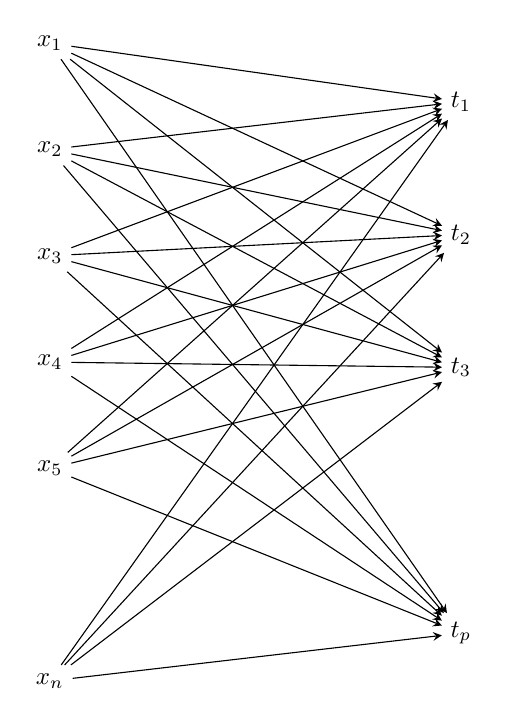
\begin{tikzpicture}[x=2.9cm, y=1.5cm, >=stealth, transform shape, scale=.9]

\foreach \m/\l [count=\y] in {1,...,5}
  \node [every neuron/.try, neuron \m/.try] (input-\m) at (0,3.5-\y) {$x_{\m}$};
  \node [neuron missing/.try] (input-missing) at (0,3.5-6) {};
  \node [every neuron/.try] (input-6) at (0,3.5-7) {$x_n$};

\foreach \h [count=\y] in {1,...,3}
  \node [every neuron/.try] (hidden-\h) at (2,3.2-\y*1.25) {$t_{\h}$};
  \node [neuron missing/.try] (hidden-missing) at (2,3.2-4*1.25) {};
  \node [every neuron/.try] (hidden-4) at (2,3.2-5*1.25) {$t_p$};

\foreach \i in {1,...,6}
  \foreach \j in {1,...,4}
    \draw [->] (input-\i) -- (hidden-\j);

\end{tikzpicture}
\caption{full connection}
\label{fig:full_con_nn}
\end{subfigure}\hfill
\begin{subfigure}[b]{.4\textwidth}
\centering
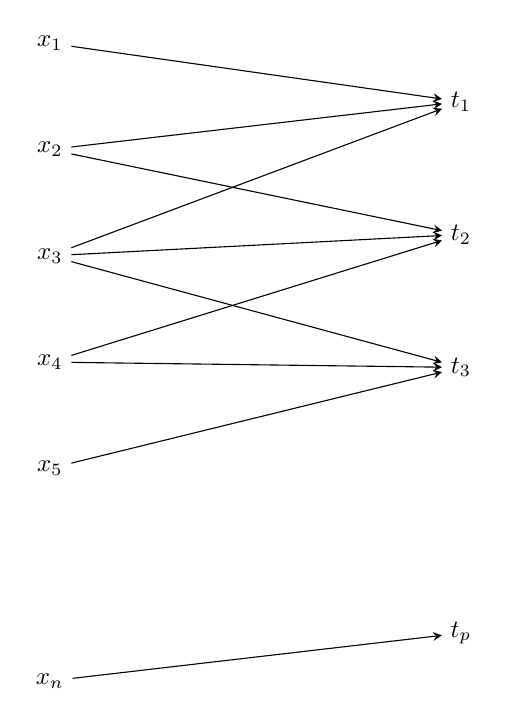
\begin{tikzpicture}[x=2.9cm, y=1.5cm, >=stealth, transform shape, scale=.9]

\foreach \m/\l [count=\y] in {1,...,5}
  \node [every neuron/.try, neuron \m/.try] (input-\m) at (0,3.5-\y) {$x_{\m}$};
  \node [neuron missing/.try] (input-missing) at (0,3.5-6) {};
  \node [every neuron/.try] (input-6) at (0,3.5-7) {$x_n$};

\foreach \h [count=\y] in {1,...,3}
  \node [every neuron/.try] (hidden-\h) at (2,3.2-\y*1.25) {$t_{\h}$};
  \node [neuron missing/.try] (hidden-missing) at (2,3.2-4*1.25) {};
  \node [every neuron/.try] (hidden-4) at (2,3.2-5*1.25) {$t_p$};

\foreach \i in {1,...,3}
    \draw [->] (input-\i) -- (hidden-1);
\foreach \i in {2,...,4}
    \draw [->] (input-\i) -- (hidden-2);
\foreach \i in {3,...,5}
    \draw [->] (input-\i) -- (hidden-3);
\draw [->] (input-6) -- (hidden-4);

\end{tikzpicture}
\caption{local connection}
\label{fig:local_con_nn}
\end{subfigure}
\caption{nn plot example}
\label{fig:nn}
\end{figure}
